% Chapter Template

\chapter{Results} % Main chapter title

\label{Chapter5} % Change X to a consecutive number; for referencing this chapter elsewhere, use \ref{ChapterX}

%----------------------------------------------------------------------------------------
%	SECTION 1
%----------------------------------------------------------------------------------------

\section{Results}
A baseline model was constructed. This model looked at the gust factor for some training data and took the average of this and predicted this average everytime. The baseline model gave an average error of around \baselineerror\%. This sets a goal. A model that does not significantly improve on this baseline suggests either failure to capture essential patterns in the data or that the data itself may lack the necessary information for substantial improvements upon the baseline. Using the previously described neural network architecture a mean absolute percentage error of \modelerror\% was achived. This is some improvement upon the baseline error, with a decrease in error of around \errorImprovement\%. The power generated by wind mill increases with wind speed cubed \cite{wind_power}. The highest wind gusts in Iceland are around 70 m/s. Knowing the gust factor to 2 percentage points better than before can allow for the anticipation power generated by wind mills in the kilowatts per square meter of swept area.

\section{Discussion}
The error improvement is modest in absolute terms but represents 21\% over the baseline. This would indicate significant improvement. A point to consider, that might heavily impact the results, is that the reanalysis data, sourced from CARRA, represents some kind of 3 hour average and therefore will be shifted towards lower values for wind speed when compared to the 10 minute measurements provided by IMO. The baseline model uses measured information to calculate the average gust factor, while the model does not have access to any measured data directly (the reanalysis data is trained on some measured data). The expected shape of the measured wind shape distribution, after filtering and nailstripping, is a bell curve with a steep tail to the right and no tail to the left and this proves to be true. If the reanalysis data would closely follow the measured wind speed, the same distribution should be observed. This is not the case. The distributions can be seen in Figure (\ref{fig:difference_measured_reanalysis})

\begin{figure}
    \centering
    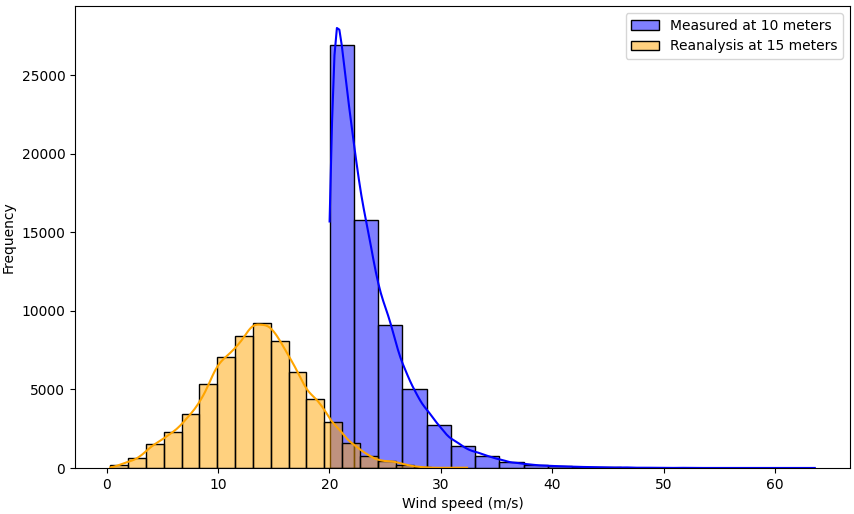
\includegraphics[scale=0.65]{Figures/difference_measured_reanalysis_cropped.png}
    \caption[Measured wind speed and corresponding points for reanalysis.]{Measured wind speed and corresponding points for reanalysis. The two distributions vary greatly. Some variation is expected, as the reanalysis represents some kind of average.}
    \label{fig:difference_measured_reanalysis}
\end{figure}

Using any information from the measurement data to improve the data, would induce data leakage. Any simple mathematical transform would not be expected to help the model as the model would simply be able to learn the pattern. A simple check was done to confirm this. The reanalysis wind speed was transformed using code shown code listing \ref{code:custom_distribution_transform}.

\begin{lstlisting}[style = Python, caption = {Custom transform method}, label = code:custom_distribution_transform]
    def custom_distribution_transform(x, threshold=20):
        max_decay, max_growth = 1.2, 6
        decay = lambda z: 1 + (max_decay-1) 
            * np.exp(threshold - z)
        growth = lambda z: 1 + (max_growth - 1) 
            * np.exp(z - threshold)
        amplification_factors = np.where(x <= threshold,
             growth(x), decay(x))
        y = amplification_factors * x + 8
        return y
\end{lstlisting}

This shift changes the shape of the reanalysis data distribution and shifts it to the right. The updated distribution can be seen in Figure (\ref{fig:transformed_reanalysis_measured}).

\begin{figure}
    \centering
    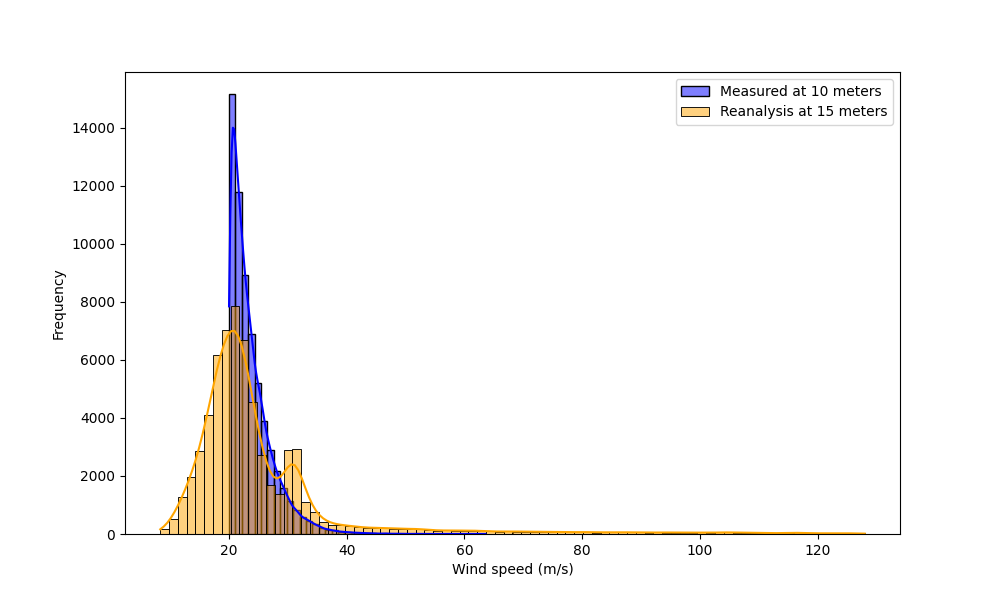
\includegraphics[scale = 0.5]{Figures/transformed_reanalysis_measured.png}
    \caption[Transformed reanalysis wind speed and measured wind speed.]{The distributions of the transformed 15 meter height wind speed of reanalysis data, along with the 10 meter measured wind speed.}
    \label{fig:transformed_reanalysis_measured}
\end{figure}

Training two identical models, one with the transformed reanalysis data and the other with original reanalysis data, results in two near identical errors, as expected. As no new information was input, the data was only manipulated, the model evaluates to the same error. The model that used the transformed reanalysis data was slightly quicker to converge.

Looking only at the error, the performance of the model can be gauged. However it does not help us explain why the model made these predictions. Here feature interpretation can be of great help. Using Shapley values and the python SHAP package, the contribution of each attribute can be given a value, as previously mentioned. Figure \ref{fig:SHAP_final_model} shows the average contribution of each feature.